\documentclass{tufte-handout}\usepackage[]{graphicx}\usepackage[]{xcolor}
% maxwidth is the original width if it is less than linewidth
% otherwise use linewidth (to make sure the graphics do not exceed the margin)
\makeatletter
\def\maxwidth{ %
  \ifdim\Gin@nat@width>\linewidth
    \linewidth
  \else
    \Gin@nat@width
  \fi
}
\makeatother

\definecolor{fgcolor}{rgb}{0.345, 0.345, 0.345}
\newcommand{\hlnum}[1]{\textcolor[rgb]{0.686,0.059,0.569}{#1}}%
\newcommand{\hlstr}[1]{\textcolor[rgb]{0.192,0.494,0.8}{#1}}%
\newcommand{\hlcom}[1]{\textcolor[rgb]{0.678,0.584,0.686}{\textit{#1}}}%
\newcommand{\hlopt}[1]{\textcolor[rgb]{0,0,0}{#1}}%
\newcommand{\hlstd}[1]{\textcolor[rgb]{0.345,0.345,0.345}{#1}}%
\newcommand{\hlkwa}[1]{\textcolor[rgb]{0.161,0.373,0.58}{\textbf{#1}}}%
\newcommand{\hlkwb}[1]{\textcolor[rgb]{0.69,0.353,0.396}{#1}}%
\newcommand{\hlkwc}[1]{\textcolor[rgb]{0.333,0.667,0.333}{#1}}%
\newcommand{\hlkwd}[1]{\textcolor[rgb]{0.737,0.353,0.396}{\textbf{#1}}}%
\let\hlipl\hlkwb

\usepackage{framed}
\makeatletter
\newenvironment{kframe}{%
 \def\at@end@of@kframe{}%
 \ifinner\ifhmode%
  \def\at@end@of@kframe{\end{minipage}}%
  \begin{minipage}{\columnwidth}%
 \fi\fi%
 \def\FrameCommand##1{\hskip\@totalleftmargin \hskip-\fboxsep
 \colorbox{shadecolor}{##1}\hskip-\fboxsep
     % There is no \\@totalrightmargin, so:
     \hskip-\linewidth \hskip-\@totalleftmargin \hskip\columnwidth}%
 \MakeFramed {\advance\hsize-\width
   \@totalleftmargin\z@ \linewidth\hsize
   \@setminipage}}%
 {\par\unskip\endMakeFramed%
 \at@end@of@kframe}
\makeatother

\definecolor{shadecolor}{rgb}{.97, .97, .97}
\definecolor{messagecolor}{rgb}{0, 0, 0}
\definecolor{warningcolor}{rgb}{1, 0, 1}
\definecolor{errorcolor}{rgb}{1, 0, 0}
\newenvironment{knitrout}{}{} % an empty environment to be redefined in TeX

\usepackage{alltt}

%\geometry{showframe}% for debugging purposes -- displays the margins

\usepackage{amsmath}
\usepackage{natbib}
\bibfont{\small} % Doesn't see to work...

% Set up the images/graphics package
\usepackage{graphicx}
\setkeys{Gin}{width=\linewidth,totalheight=\textheight,keepaspectratio}
% \graphicspath{{graphics/}}
\title{Introducing of R: Temperature vs. Depth %\thanks{}
}
\author[Marc Los Huertos]{Marc Los Huertos}
\date{}  % if the \date{} command is left out, the current date will be used


% \SweaveOpts{prefix.string=graphics/plot} % Created a "graphics" subdirectory to 

\setsidenotefont{\color{blue}}
% \setcaptionfont{hfont commandsi}
% \setmarginnotefont{\color{blue}}
% \setcitationfont{\color{gray}}

% The following package makes prettier tables.  We're all about the bling!
\usepackage{booktabs}

% Small sections of multiple columns
\usepackage{multicol}
\IfFileExists{upquote.sty}{\usepackage{upquote}}{}
\begin{document}

\maketitle% this prints the handout title, author, and date
\begin{abstract}
\noindent R is a robust, open source software package to process and analyzed data. As an extremely flexible programming environment, its development has been rapid and popularity has been growing dramatically in recent years. Most graduate schools teach R and many are phasing out the traditional software package site licenses (\eg SAS, SPSS, etc). 

This handout provides an brief introduction to the syntax of R and some applications to plot and bivariate data. I believe R provides a mechanism to learn 1) skills to process electronic data, 2) a programming environment to implement a range of statistical tests, and 3) provide skills that can be used in your future career, whether or not R is used again.\sidenote{Typeset using the Sweave function in R and \LaTeX\ using a \citet{Tufte:1983, Tufte:1997} and style.}
\end{abstract}

% Setting up the margins, etc for R


\section{Session Goals}

\begin{enumerate}
	\item Open and use the R GUI with consistent results.
	\item Use math operators to solve simple calculations.
	\item Create vectors (type of objects).
	\item Best fit line and linear models.
\end{enumerate}

\section{The R GUI}

Starting the program is fairly easy.\sidenote[][-.5in]{Outcome: Open R and use the R GUI with consistent results.} Assuming R is installed,\footnote[][.03in]{If R is not installed, it can be done easily by going to http://www.r-project.org/ and downloading the free software "base" program, which have been compiled for Windows and Mac and there is source code for Linux and Unix boxes.} find R by going to the windows "Start" button, navigate to "All Programs" and search for "R". Click on R program, whose icon is usually an capital R followed by a version number. 

Now that R is started, you should notice a few things.  The GUI, or graphical user interface is quite Spartican, compared to what computers are capable of. For beginners this is the most disturbing part of the program. Second, there are some hints of how to start, but to follow these hints, you have to type exactly what you see. Yes, computers are stupid, they only recognized the commands they expect, not what you want them to understand. 

\begin{figure}
		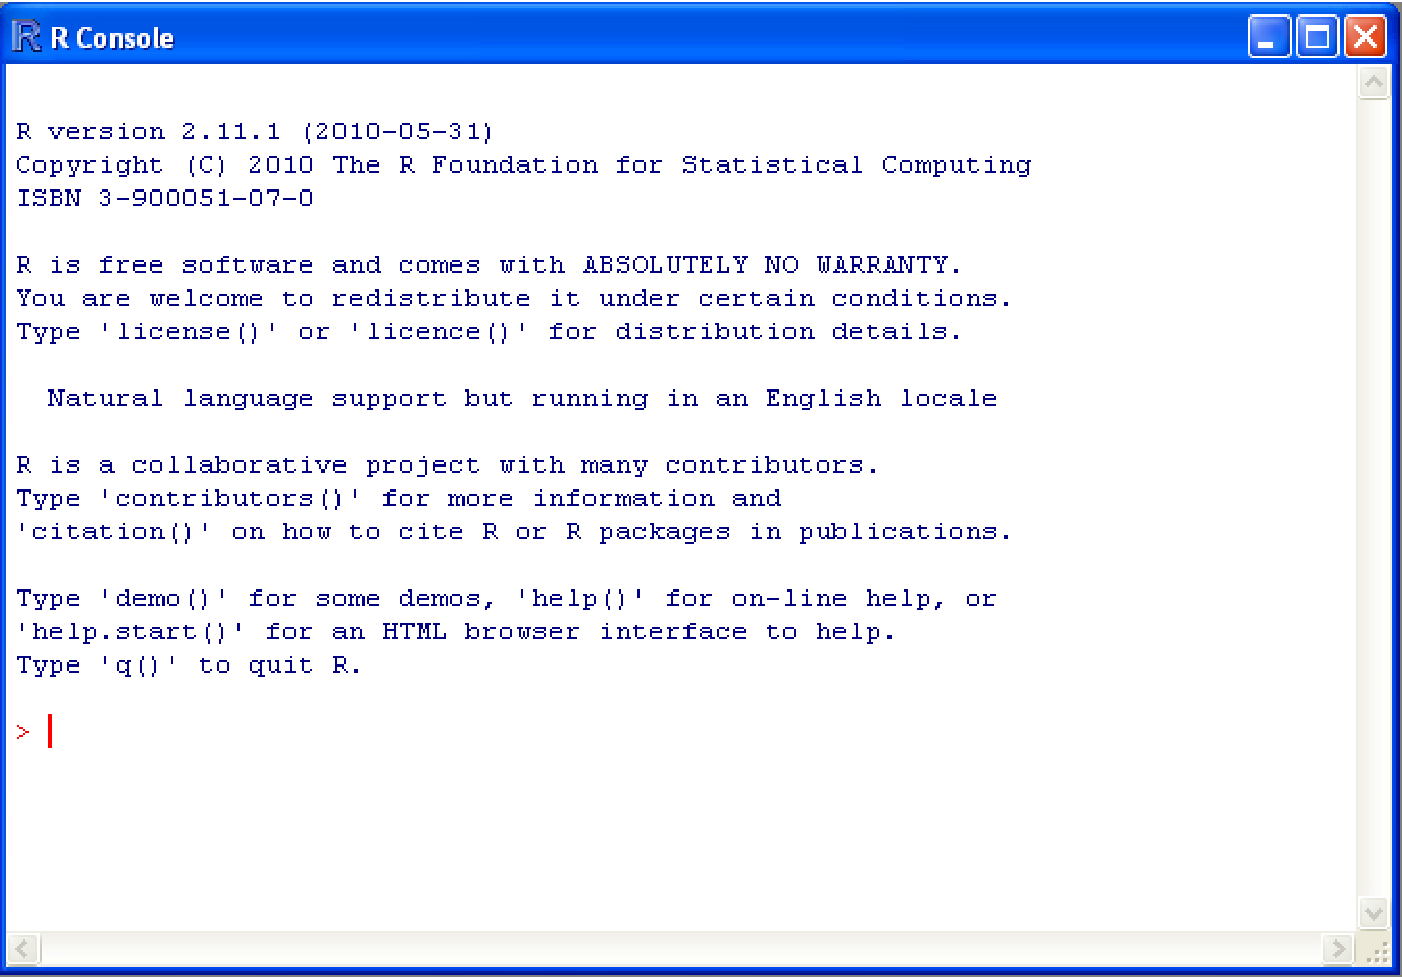
\includegraphics{OpeningScreenShot.pdf}
	\caption{Opening window screen shot of R. Notice the version number is probably different than what you have. Don't worry about this, the differences are minor and only play a significant role as you start to do more advanced statistics. There are new versions every few months and I might be a few versions ahead or behind what you see. Also, notice some hints have been created for the beginner. However, you much type exactly what you see including the parentheses. Most commands in R have parentheses, which signifies a function, which are like verbs in R. Without a function (or verb), R doesn't really know what to do.}
	\label{fig:OpeningScreenShot}
\end{figure}

At the bottom of the screen is a prompt, which is a ">" symbol. Yes, you could change that to something more recognizable, but later you will appreciate the simplicity. This is where R expects commands lines to be entered. This characteristic is why R is called a command line program. There are no buttons to push and the menus are pretty limited.
  
Let's start with closing R.  Type "quit()" to close R. Notice that R asked you to save the workspace. R keeps track of your typing history and objects that you create. I'll explain objects soon enough. I generally don't save anything, if you do, you might find a bewildering number of objects that will interfere with your work at a later date. So, click "no" and R goes away.

Start R again. Congratulations, you have just met the first outcome. You can smile and get a drink of water.

Before moving on, open a word processor and begin recording your response to following question and question at the end of each section.

\bigskip
\noindent \textbf{\#1 Please list three or four questions you have so far. }

\section{R as a Calculator}

Using a computer for calculating values has become a trivial exercise with the widespread use of Excel.\sidenote{Outcome: Use math operators to solve simple calculations.} However, there are a number of symbols required when you are doing math functions on a computer because the keyboard is not specialized like a calculator. Thus, we have to learn how to use operators using simple keyboard characters. See the Table~\ref{tab:KeyboardOperators} for a list of the common characters used for operators in R.

\begin{table}
	\begin{center}
	\begin{tabular}{lcc}
		\toprule
Operation &\ Operator &\ Example \\
\midrule
Addition & + &  6 + 5  \\  
Subtraction & - & 6 - 5 \\
Multiplication & * & 6 * 5 \\
Division & / & 3 / 5\\
Power & $\wedge$ & 3 $\wedge$ 5  \\
\bottomrule
\end{tabular}
\end{center}	
\caption{Keyboard Operator for Mathematical Operations in R.}
	\label{tab:KeyboardOperators}
\end{table}

In addition, for more complex operations, R uses functions, which have a different syntax, \eg \texttt{log()}, \texttt{exp()}, \texttt{sin()}, etc. The syntax for these functions is fairly straightforward. For example, to calculate the base 10 logarithm of 3.5, we can type:\sidenote{as below, each time you see a ``>'', I am referring to the R prompt and you want to type the text after the prompt.}

\begin{knitrout}
\definecolor{shadecolor}{rgb}{0.969, 0.969, 0.969}\color{fgcolor}\begin{kframe}
\begin{alltt}
\hlkwd{log10}\hlstd{(}\hlnum{3.5}\hlstd{)}
\end{alltt}
\begin{verbatim}
## [1] 0.544068
\end{verbatim}
\end{kframe}
\end{knitrout}

Or to calculate the natural log, type
\begin{knitrout}
\definecolor{shadecolor}{rgb}{0.969, 0.969, 0.969}\color{fgcolor}\begin{kframe}
\begin{alltt}
\hlkwd{log}\hlstd{(}\hlnum{3.5}\hlstd{)}
\end{alltt}
\begin{verbatim}
## [1] 1.252763
\end{verbatim}
\end{kframe}
\end{knitrout}

R allows the user to make complex equations and even solving complex calculations. For example, the if you want to solve the following equation:

\begin{equation}
V = V_{max}\frac{S}{K_s + S}
\end{equation}

And $V_{max}$ = 3, $S$ = 1.0 and $K_s = 0.3$, then you can type

\begin{knitrout}
\definecolor{shadecolor}{rgb}{0.969, 0.969, 0.969}\color{fgcolor}\begin{kframe}
\begin{alltt}
\hlnum{3.0} \hlopt{*} \hlstd{(}\hlnum{1.0} \hlopt{/} \hlstd{(}\hlnum{0.3} \hlopt{+} \hlnum{1.0}\hlstd{))}
\end{alltt}
\begin{verbatim}
## [1] 2.307692
\end{verbatim}
\end{kframe}
\end{knitrout}

However, typing these formulas can be time consuming and subject to typos, (\eg it is easy to forget to put the parentheses in the right place) so we'll see how we can streamline the process to make R uses more efficient. 

\bigskip
\noindent \textbf{\#2 What are the differences between what you have seen in other computer programs so far? }

\section{Objects in R}

\subsection{Creating Objects}

Typing a long string of numbers each time you want to due something is a waste of time and effort. Let's say you wanted to have the numbers from 1 to 10. But R would have no way to handle this series. Instead, we use R to store these values in an object and recall them at will. To create objects in R, we use either the \texttt{=} or the \texttt{<-} symbols, which is composed of a ``less than symbol'' and a ``dash.'' I prefer the second because it is obviously directional and thus there is no ambiguity.\sidenote{Outcome: Create Objects.}

When creating an object, we need to name the object and define the object type. Usually, this can be done in a single step. But we'll try to break it down so you can follow along. First, let's say we want to make an object that has 10 numbers in it. The most basic type of object is a vector, which can store a string of numbers or characters. Let's call the vector something recognizable, \texttt{myvector}. To put numbers into a vector, we need to concatenate or combine them, thus we need R to do something with the numbers, in other words, we need a "verb". In this case the verb concatenate or combine is abbreviated as \texttt{c()}. Remember with each function, there are parentheses. Now what we put ten numbers into the parentheses to be concatenated. We'll put a series of numbers from 1 to 10. 

\begin{knitrout}
\definecolor{shadecolor}{rgb}{0.969, 0.969, 0.969}\color{fgcolor}\begin{kframe}
\begin{alltt}
\hlstd{myvector} \hlkwb{<-} \hlkwd{c}\hlstd{(}\hlnum{1}\hlstd{,} \hlnum{2}\hlstd{,} \hlnum{3}\hlstd{,} \hlnum{4}\hlstd{,} \hlnum{5}\hlstd{,} \hlnum{6}\hlstd{,} \hlnum{7}\hlstd{,} \hlnum{8}\hlstd{,} \hlnum{9}\hlstd{,} \hlnum{10}\hlstd{)}
\end{alltt}
\end{kframe}
\end{knitrout}

In this case, each number to be combined is separated by a comma. Spaces between the commas does not affect the object at all. Notice when you create the vector, R does not return any response. At first, this might seem disconcerting. But soon, you will be excited by the silence. In general, no news is good news in R, i.e. when there is no response, R did something and there was no error. Now it might not be what you wanted, but it did something. So, now let's see if R did what we wanted. 

Now, we can view the vector by typing the name of the vector as below:\sidenote{The numbers in the square brackets are referencing the "index" number of the first observation in the row. It will make more sense when we create longer vectors.}  

\begin{knitrout}
\definecolor{shadecolor}{rgb}{0.969, 0.969, 0.969}\color{fgcolor}\begin{kframe}
\begin{alltt}
\hlstd{myvector}
\end{alltt}
\begin{verbatim}
##  [1]  1  2  3  4  5  6  7  8  9 10
\end{verbatim}
\end{kframe}
\end{knitrout}

\subsection{Interrogating Objects}

We now use a function to interrogate the vector. For example, how long is the vector?

\begin{knitrout}
\definecolor{shadecolor}{rgb}{0.969, 0.969, 0.969}\color{fgcolor}\begin{kframe}
\begin{alltt}
\hlkwd{length}\hlstd{(myvector)}
\end{alltt}
\begin{verbatim}
## [1] 10
\end{verbatim}
\end{kframe}
\end{knitrout}

What is the sum of the values in the vector?

\begin{knitrout}
\definecolor{shadecolor}{rgb}{0.969, 0.969, 0.969}\color{fgcolor}\begin{kframe}
\begin{alltt}
\hlkwd{sum}\hlstd{(myvector)}
\end{alltt}
\begin{verbatim}
## [1] 55
\end{verbatim}
\end{kframe}
\end{knitrout}

What is the mean of the vector?

\begin{knitrout}
\definecolor{shadecolor}{rgb}{0.969, 0.969, 0.969}\color{fgcolor}\begin{kframe}
\begin{alltt}
\hlkwd{mean}\hlstd{(myvector)}
\end{alltt}
\begin{verbatim}
## [1] 5.5
\end{verbatim}
\end{kframe}
\end{knitrout}

Congratulations, you have now made an object. This object is a vector, which we  named "myvector".\footnote{By the way, R is case sensitive, so "myvector" or "myVector" or "Myvector" refer to two different objects, two of which don't exists. Failing to keep track of what is upper and lower case can lead to high levels of frustration. I suggest you start with keeping everything lower case to avoid confusion. However, I will violate this suggestion immediately, for reasons that I will explain below.} Another thing to notice is that we have created a vector of numbers, would have also created a vector of characters (and words) and logical or binary responses, \ie TRUE and FALSE.

\bigskip
\noindent \textbf{\#3 Please list what questions might have come up in this section? }

\subsection{Types of Objects}

There a variety of objects that can be created in R (Table~\ref{tab:CommonObjects}). For the purpose of our class, we will concentrate on the following objects:
\begin{table}
	\centering
		\begin{tabular}{ll}
Object Type &\ Coercive functions \\
\hline
Vector & \texttt{c()}, \texttt{as.vector()} \\
Matrix & \texttt{matrix()}, \texttt{as.matrix()} \\
List & \texttt{list()}, \texttt{as.list()} \\
Data frame & \texttt{data.frame()}, \texttt{as.data.frame()} \\
Linear model & \texttt{lm()}, \texttt{aov()} \\\hline
		\end{tabular}
	\caption{Examples of common objects and the coercive functions to create them. We will use many of these, so do not worry if you don't know what they mean yet.}
	\label{tab:CommonObjects}
\end{table}



Okay, we have dumped the each of the treatments onto the screen, but we haven't created any objects. Next, create a vector of the 15 observations, but using the c() function, which combines or more accurately concatenates the values. 

\begin{knitrout}
\definecolor{shadecolor}{rgb}{0.969, 0.969, 0.969}\color{fgcolor}\begin{kframe}
\begin{alltt}
\hlstd{temperature} \hlkwb{=} \hlkwd{c}\hlstd{(}\hlnum{15}\hlstd{,} \hlnum{15}\hlstd{,} \hlnum{14}\hlstd{,} \hlnum{12}\hlstd{,} \hlnum{12}\hlstd{,} \hlnum{10}\hlstd{)}
\hlstd{depth} \hlkwb{=} \hlkwd{c}\hlstd{(}\hlnum{2}\hlstd{,} \hlnum{4}\hlstd{,} \hlnum{6}\hlstd{,} \hlnum{8}\hlstd{,} \hlnum{10}\hlstd{,} \hlnum{12}\hlstd{)}
\end{alltt}
\end{kframe}
\end{knitrout}

There are a few things to notice. First, look at all the parentheses. Keeping track of these is really important, for every opening parentheses there is a closing one. And they have to be in the right place, based on the syntax of the function. As you can see, this can get rather complicated and mistakes will be made. In other words, try to pay attention to these characters, and if you get errors, look for mistakes with parenthesis as first strategy to fix errors. Second, notice all the commas. Just as important to the syntax of these commands as parenthesis, commas need to be in the right place. If they are not, you will get errors. Remember, no news is good news in R; when you get some text in return that you haven't asked for, there is an error somewhere, and always check for commas and parenthesis firsts. Finally, failing to match opening and closing quotations marks are also a common error. 

Generate 3 different error messages by leaving out a closing parenthesis or quotation mark or comma. See what happens if you have all three errors. You can see that error trapping in R is rudimentary, so you can spend a fair amount of time deciphering errors which are actually really simple to fix. 

On of the most common objects is a data frame, which appears to be like a spreadsheet. We'll create a data frame by combining two vectors. First, let's create the vector of response values, which are flower date, as reported in Julian dates.\footnote[][-1.1cm]{Julian dates are the day number since the first day of the year, thus January 1st is Julian date 1 and Julian date 31 is January 31st.}



\begin{fullwidth}

\end{fullwidth}



The vector name is a bit long, but it describes exactly what are in the data. It seems worth having names that are meaningful and that can remembered. But there is a trade off, you have to spell it correctly, so you may prefer shorter names. 

Let's check to see if both vectors have the same length. If they are not, they will not be able to be combined into a data frame. Notice that each of the vectors have lower case letters. We could have capitalized the first letter, but as you will see below, I reserve that for data frame variable names. It is a matter of preference.

\begin{knitrout}
\definecolor{shadecolor}{rgb}{0.969, 0.969, 0.969}\color{fgcolor}\begin{kframe}
\begin{alltt}
\hlkwd{length}\hlstd{(temperature)}
\end{alltt}
\begin{verbatim}
## [1] 6
\end{verbatim}
\begin{alltt}
\hlkwd{length}\hlstd{(depth)}
\end{alltt}
\begin{verbatim}
## [1] 6
\end{verbatim}
\end{kframe}
\end{knitrout}


\section{Linear Models in R}

The use of the linear model is the cornerstone of statistics. So ubiquitous it is rarely explained coherently.\sidenote{Outcome: Build and test a linear model.} The linear model can be summarized at the equation for a line, but with the addition of error. You are probably familiar with the equation for a line where, 

\begin{equation}
y = m * x + b
\end{equation}

This equation defines a line, where $m$ is the slope, $b$ is the y-intercept, and the x and y are coordinates. The linear model is based on this form and is usually written as  

\begin{equation}
y \sim \alpha + \beta * x + \epsilon
\end{equation}

The order is usually changed, where the intercept is first, followed by the slope and x variable and the addition of error or noise. The error is usually symbolized as $\epsilon$. In general, in a statistical model, Greek letters are used and instead of an equals sign, we use a tilde, meaning that that left side of the equation is a function of the right side. Luckily, this is the approximate form that R expects, so if you understand this, you will have a pretty good idea of how to code a linear model in R. 

The function to build a linear model is \texttt{lm()}. This function is extremely powerful and can be easily implemented, but this is a good time to see what the help menus look like in R. 

\begin{knitrout}
\definecolor{shadecolor}{rgb}{0.969, 0.969, 0.969}\color{fgcolor}\begin{kframe}
\begin{alltt}
\hlkwd{help}\hlstd{(lm)}
\end{alltt}
\end{kframe}
\end{knitrout}

I am not showing it here, but you should see a long complex looking help page window pop up. All help files in R are structured the same way, so in spite of the uninterpretable text, written by and for computer programmers, the structure will become familiar. Beginning with the description, the help screen describes the function, how to use it, and give some examples. Admittedly, I rarely understand much of the text, but I find the examples to be very useful! In fact, I suggest you paste the example into R and see what happens, I find this one of the best ways to learn R. Use an example that I know works, then change it to make it do what I want it to do.

Using the linear model, we can analyze several types of data, when the response variable is continuous. If the have a predictor variable that is categorical, then we often analyze the data using the method known as analysis of variance or ANOVA. If the predictor variable is continuous, then we often analyze data using a regression analysis. 


\begin{knitrout}
\definecolor{shadecolor}{rgb}{0.969, 0.969, 0.969}\color{fgcolor}\begin{kframe}
\begin{alltt}
\hlkwd{plot}\hlstd{(depth, temperature)}
\end{alltt}
\end{kframe}
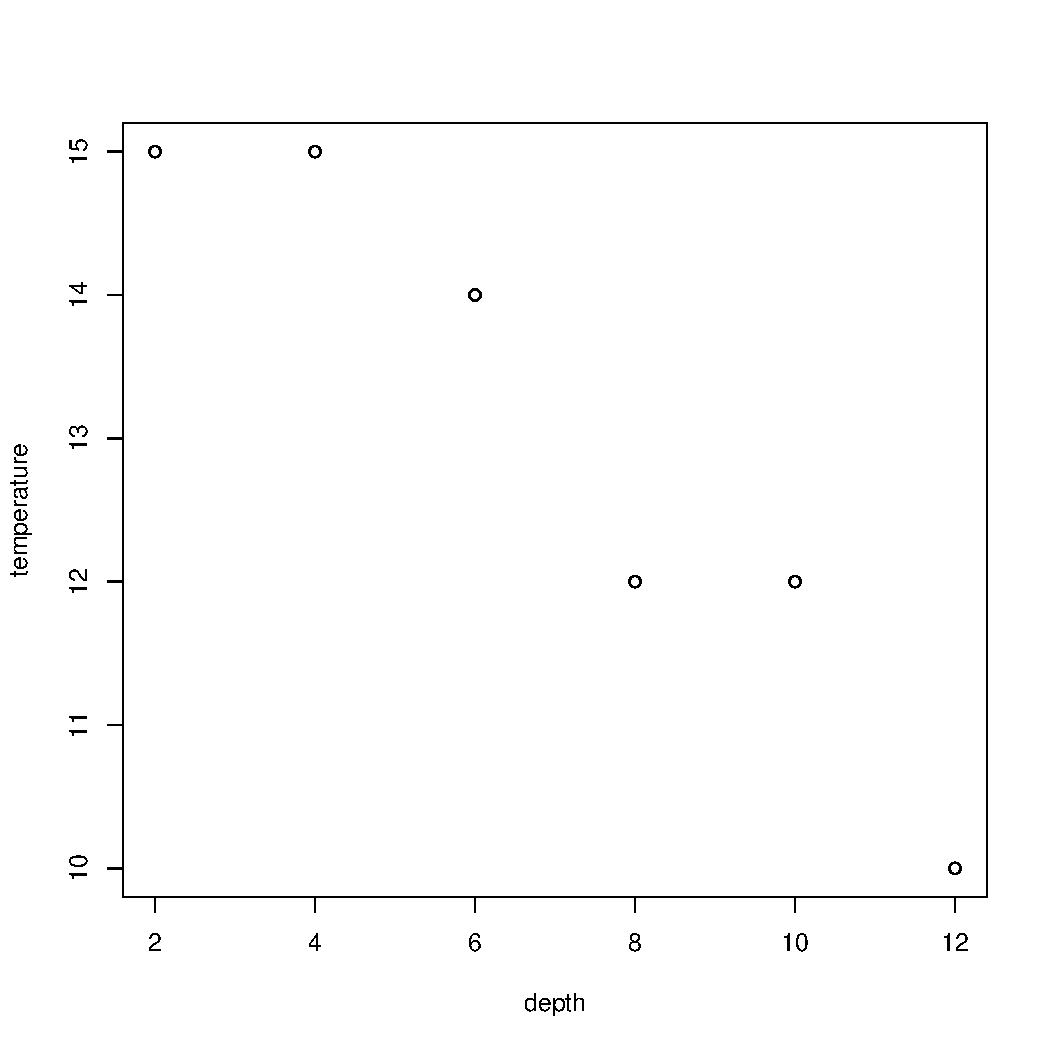
\includegraphics[width=\maxwidth]{figure/unnamed-chunk-17-1} 
\end{knitrout}

\end{document}



